%%Talk about the replication of the original experiment in a dynamic scenario

The first independent replication to collect empirical results was done with the algorithms proposed in the original work by \textit{Schwarzrock et al.}~\citep{MAS07} using the dynamic scenario presented in Section \ref{sec:dynamic_scenario}. It aims to find evidence to either support or refute the conjecture made in the referenced study that it would be fully functional in dynamic scenarios. 

Table \ref{table:table01} shows the results from all algorithms proposed by the original study~\citep{MAS07} applied to dynamic context. These results show the total reward obtained with the completed tasks, the total tasks that were finished, the portion of total time ($[0\%,1\%]$) used to perform the maximum possible tasks, the total quality that relates the sensors and the performed tasks, and the number of tokens sent during the execution of the experiments. Some results are normalized to make the comparisons easier. 

\begin{table}%[ht]
	\small
	\fontsize{6}{6}\selectfont
	\centering
	\caption{Total reward, elapsed time, quantity and quality of the completed tasks and number of exchanged messages(tokens sent) for 100 runs of each algorithm with the following attributes: 9 UAVs and 96 tasks in area of 300x240 pixels with deadline of 300 ticks.}
	\label{table:table01}
	
	\begin{tabular}{rrrrr} \hline
		& AL
		& SAL
		& LAL \\ \hline 
		
		& Mean (St.Dev.)  & Mean (St.Dev.)  & Mean (St.Dev.)  \\ [1ex]
		
		\multicolumn{5}{l}{\textbf{Results of the reference study in the same original static context}} \\
	Total reward           & 16.724   ($\pm$2.1908)  & 37.9608  ($\pm$1.1119) & 44.733  ($\pm$1.5961)   \\
	Elapsed time (norm)    & 0.9894   ($\pm$0.0064)  &  0.9763  ($\pm$0.0092) & 0.9693  ($\pm$0.0124)    \\ 
	Comp. tasks (norm)     & 0.2774   ($\pm$0.0276)  &  0.4674  ($\pm$0.0170) & 0.5226  ($\pm$0.0162)    \\ 
	Quality (norm)         & 0.7865   ($\pm$0.0641)  &  0.9680  ($\pm$0.0202) & 0.9752  ($\pm$0.0159)   \\ 
	Sending token          &  9.8667  ($\pm$1.1958)  &  9.7000  ($\pm$1.2360) & 51.500 ($\pm$1.4797)   \\ [1ex]
		
		\multicolumn{5}{l}{\textbf{Independent replication using the dynamic context (number of UAVs changes)}} \\
	Total reward           & 8.6995  ($\pm$1.9489)  & 23.6496 ($\pm$2.6004) &  28.348  ($\pm$2.8464)  \\
	Elapsed time (norm)    & 0.9767  ($\pm$0.0135)  & 0.9652  ($\pm$0.0220) &  0.9513  ($\pm$0.0281)  \\ 
	Comp. tasks (norm)     & 0.1418  ($\pm$0.0281)  & 0.2852  ($\pm$0.0315) &  0.3278  ($\pm$0.0328)  \\ 
	Quality (norm)         & 0.5753  ($\pm$0.1421)  & 0.5751  ($\pm$0.1358) &  0.5858  ($\pm$0.1424)  \\ 
	Sending token          & 10.0900 ($\pm$1.3416)  & 9.9800  ($\pm$1.1805) &  49.4600 ($\pm$1.9562)  \\ [1ex]

		\hline
	\end{tabular}
\end{table} 






The analysis concentrates in all results of the experiments that used more agents (9 UAVs) and tasks (96) since they represent the highest value difference between the dependent variables of the original study and those obtained in the dynamic scenario. All other results are available in the repository\footnote{https://github.com/junieramorim/replicationMaterial}. Overall, these results suggest that the original algorithms work in a dynamic scenario due to the average level obtained with no inconsistent value to all variables, e.g., zero or negative values. Nevertheless, those results were significantly different from the values obtained by the original work.

Graphs comparing the results obtained with this first replication in the dynamic scenario (Section \ref{sec:dynamic_scenario}) and the reproduction of original study in the static context are presented in the following, along with a related discussion.

The metric concerning the number of finished tasks (Figure \ref{fig:fig04}) presented a reduction greater than $40\%$ due to the fact that there are fewer agents performing the mission. Indeed, as the dynamic scenario makes the number of agents decreases at runtime, not all tasks allocated are completed, which explains this difference. 

Another metric that suffered a significant degradation (greater than $30\%$) was the quality, as seen in Figure \ref{fig:fig03}. This quality is calculated as a sum of the sensors compatibility with the tasks, i.e., each sensor has a number between 0 and 1 that defines how suitable this sensor is to be used in a specific task, correlating the sensors characteristics and the type of task. This number ($Q_{ij}$) defines the agent $i$ quality to perform the task $j$ and it is used to calculate the agent capability ($k_{ij}$) (Equation \ref{eq:capability}).

The reduction in this attribute was in consequence of the algorithms characteristics that simply discard the allocated tasks, from the available tasks list, when the agent is shut down. These tasks are not reallocated among the remaining UAVs, thus reducing the quality of the sensors related to the finished tasks.

\begin{figure}[h!]
	\begin{center}
		%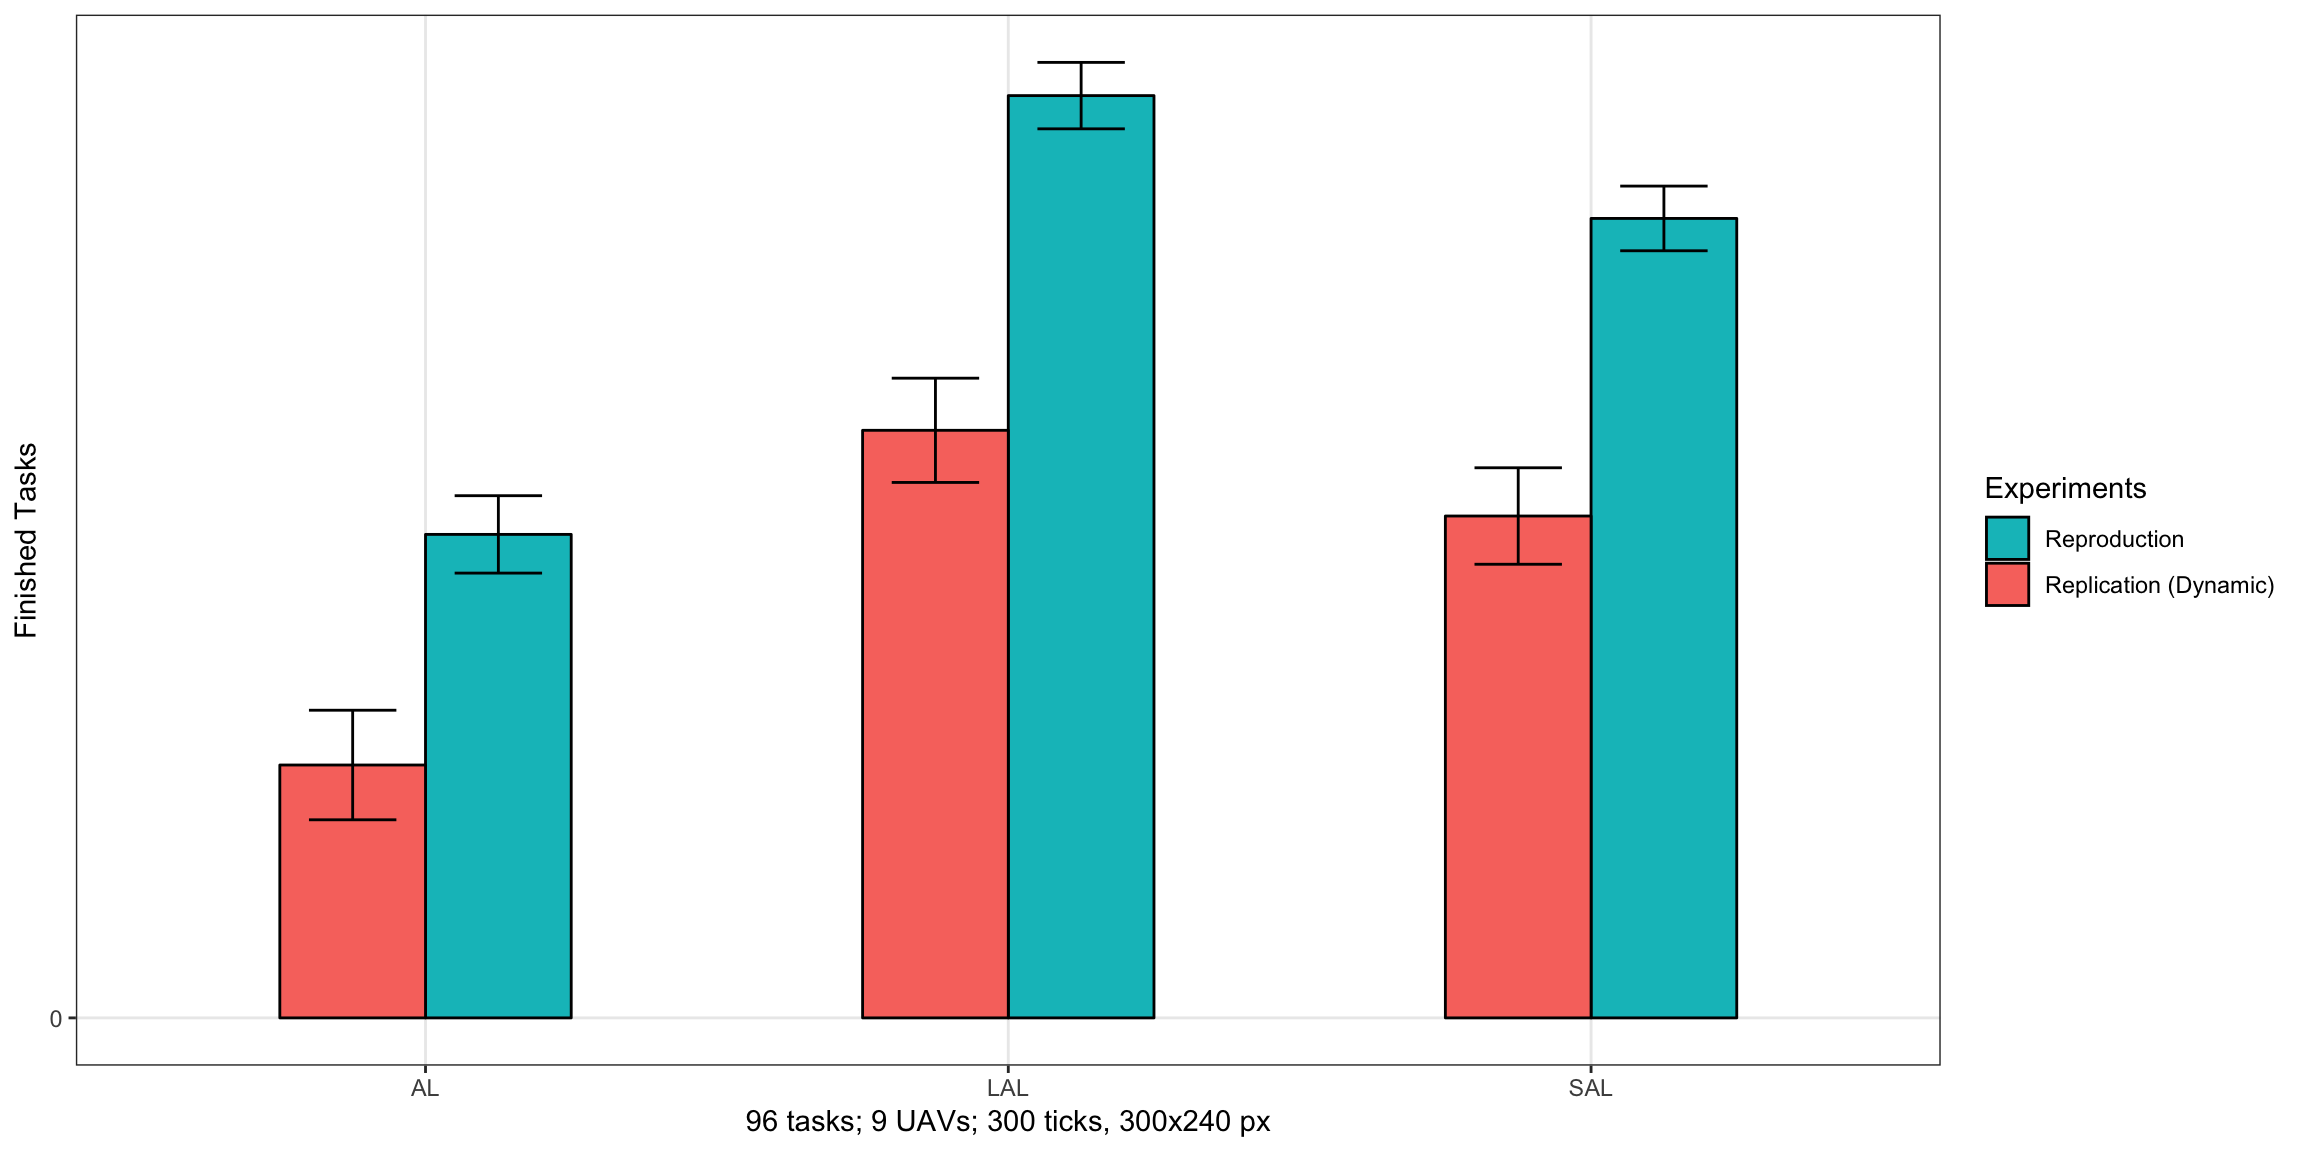
\includegraphics[scale=0.15]{fig/finished_orig.png}
		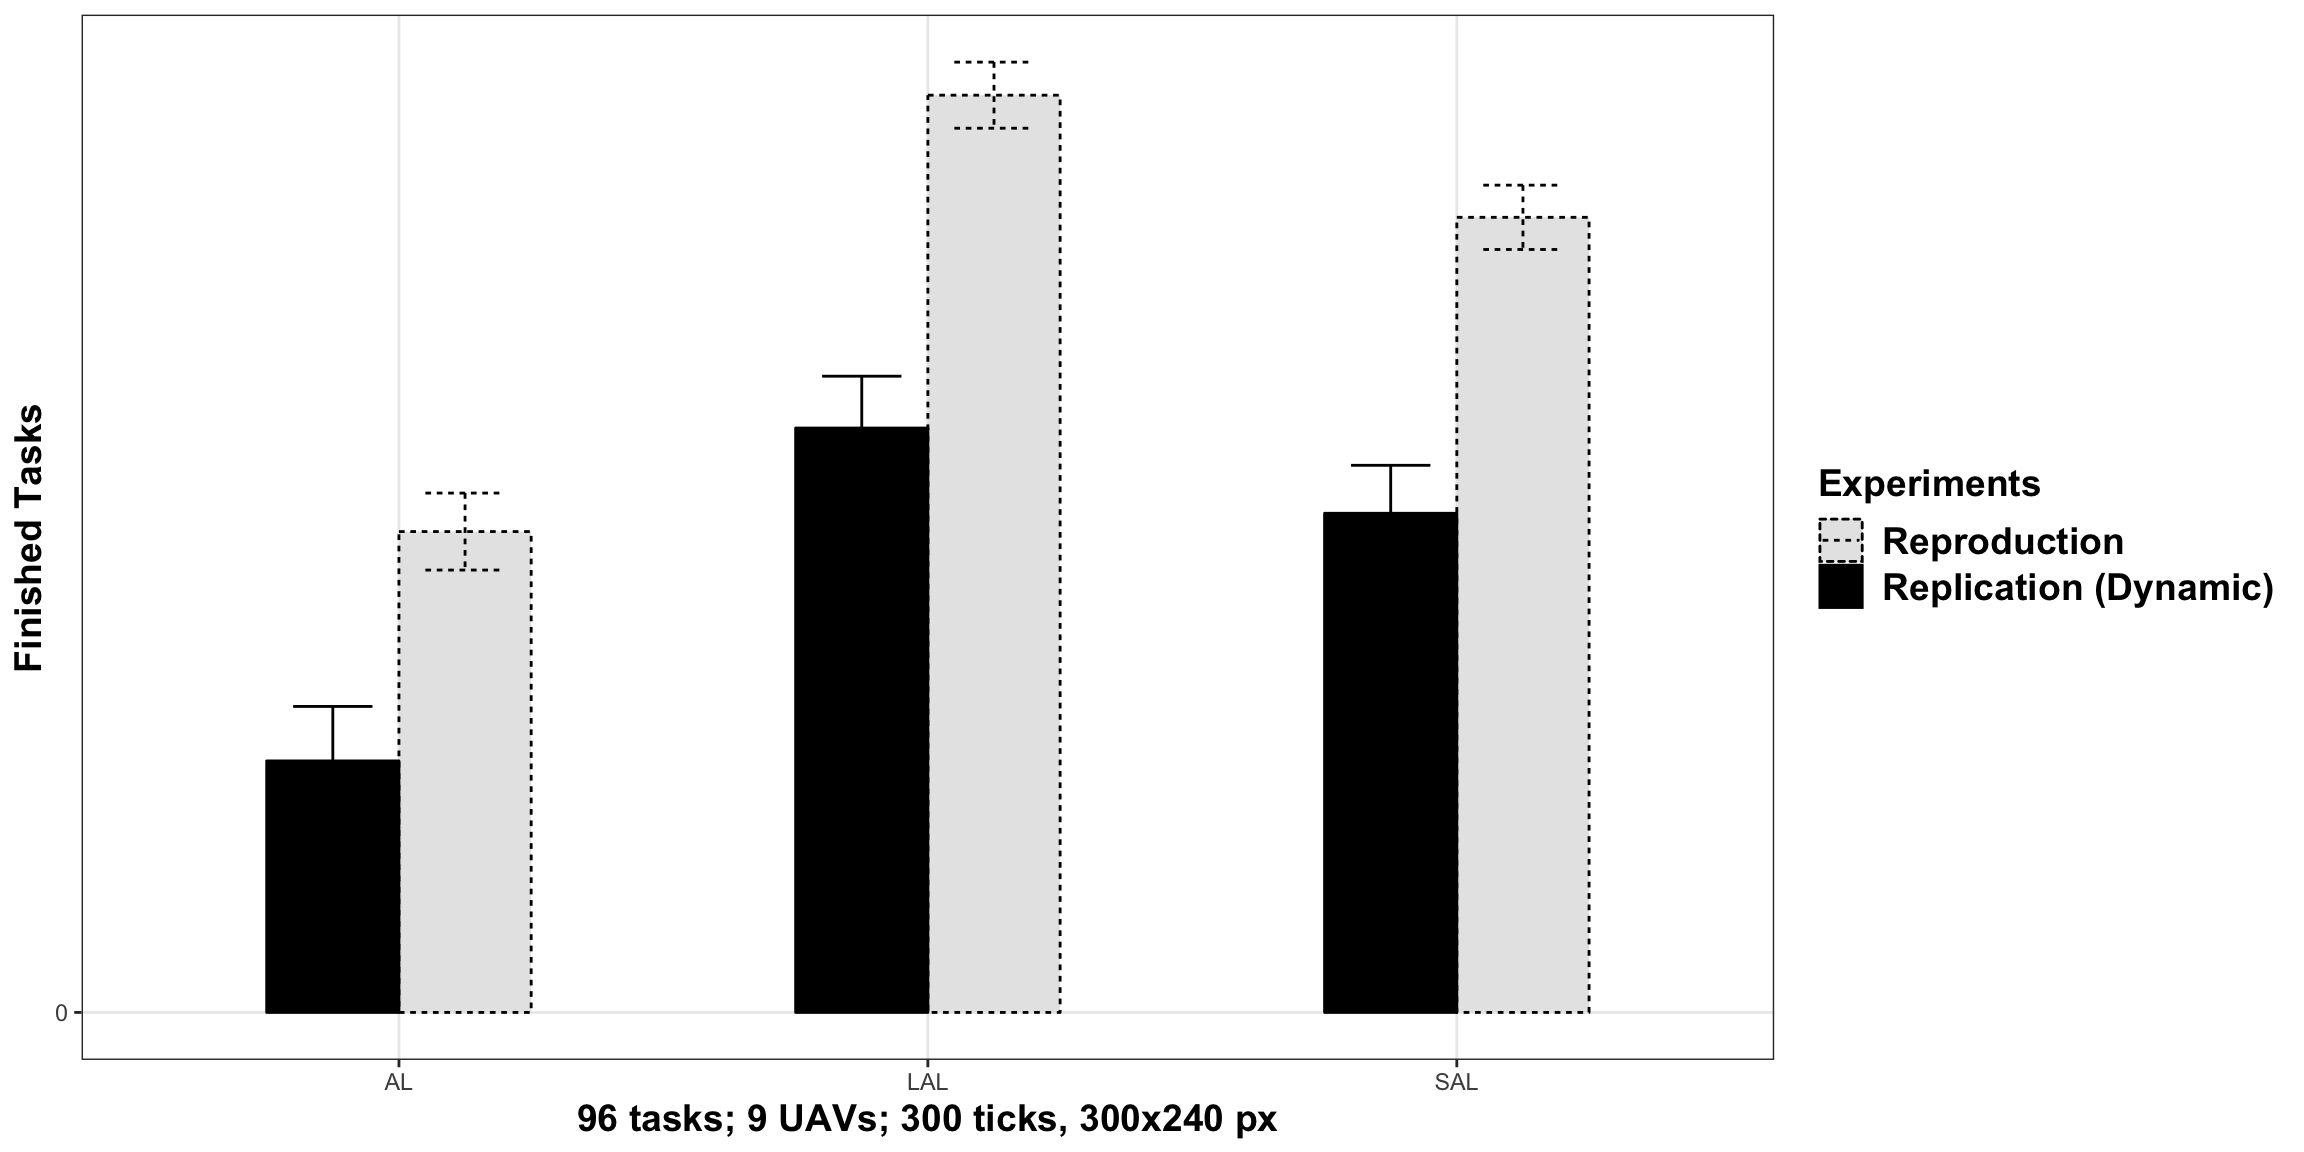
\includegraphics[scale=0.15]{fig/GRAPH01.png}
		\caption{Finished Tasks (96 tasks; 9 UAVs; 300 x 240; 300 ticks)}
		\label{fig:fig04}
	\end{center}
\end{figure}

\begin{figure}[h!]
	\begin{center}
		%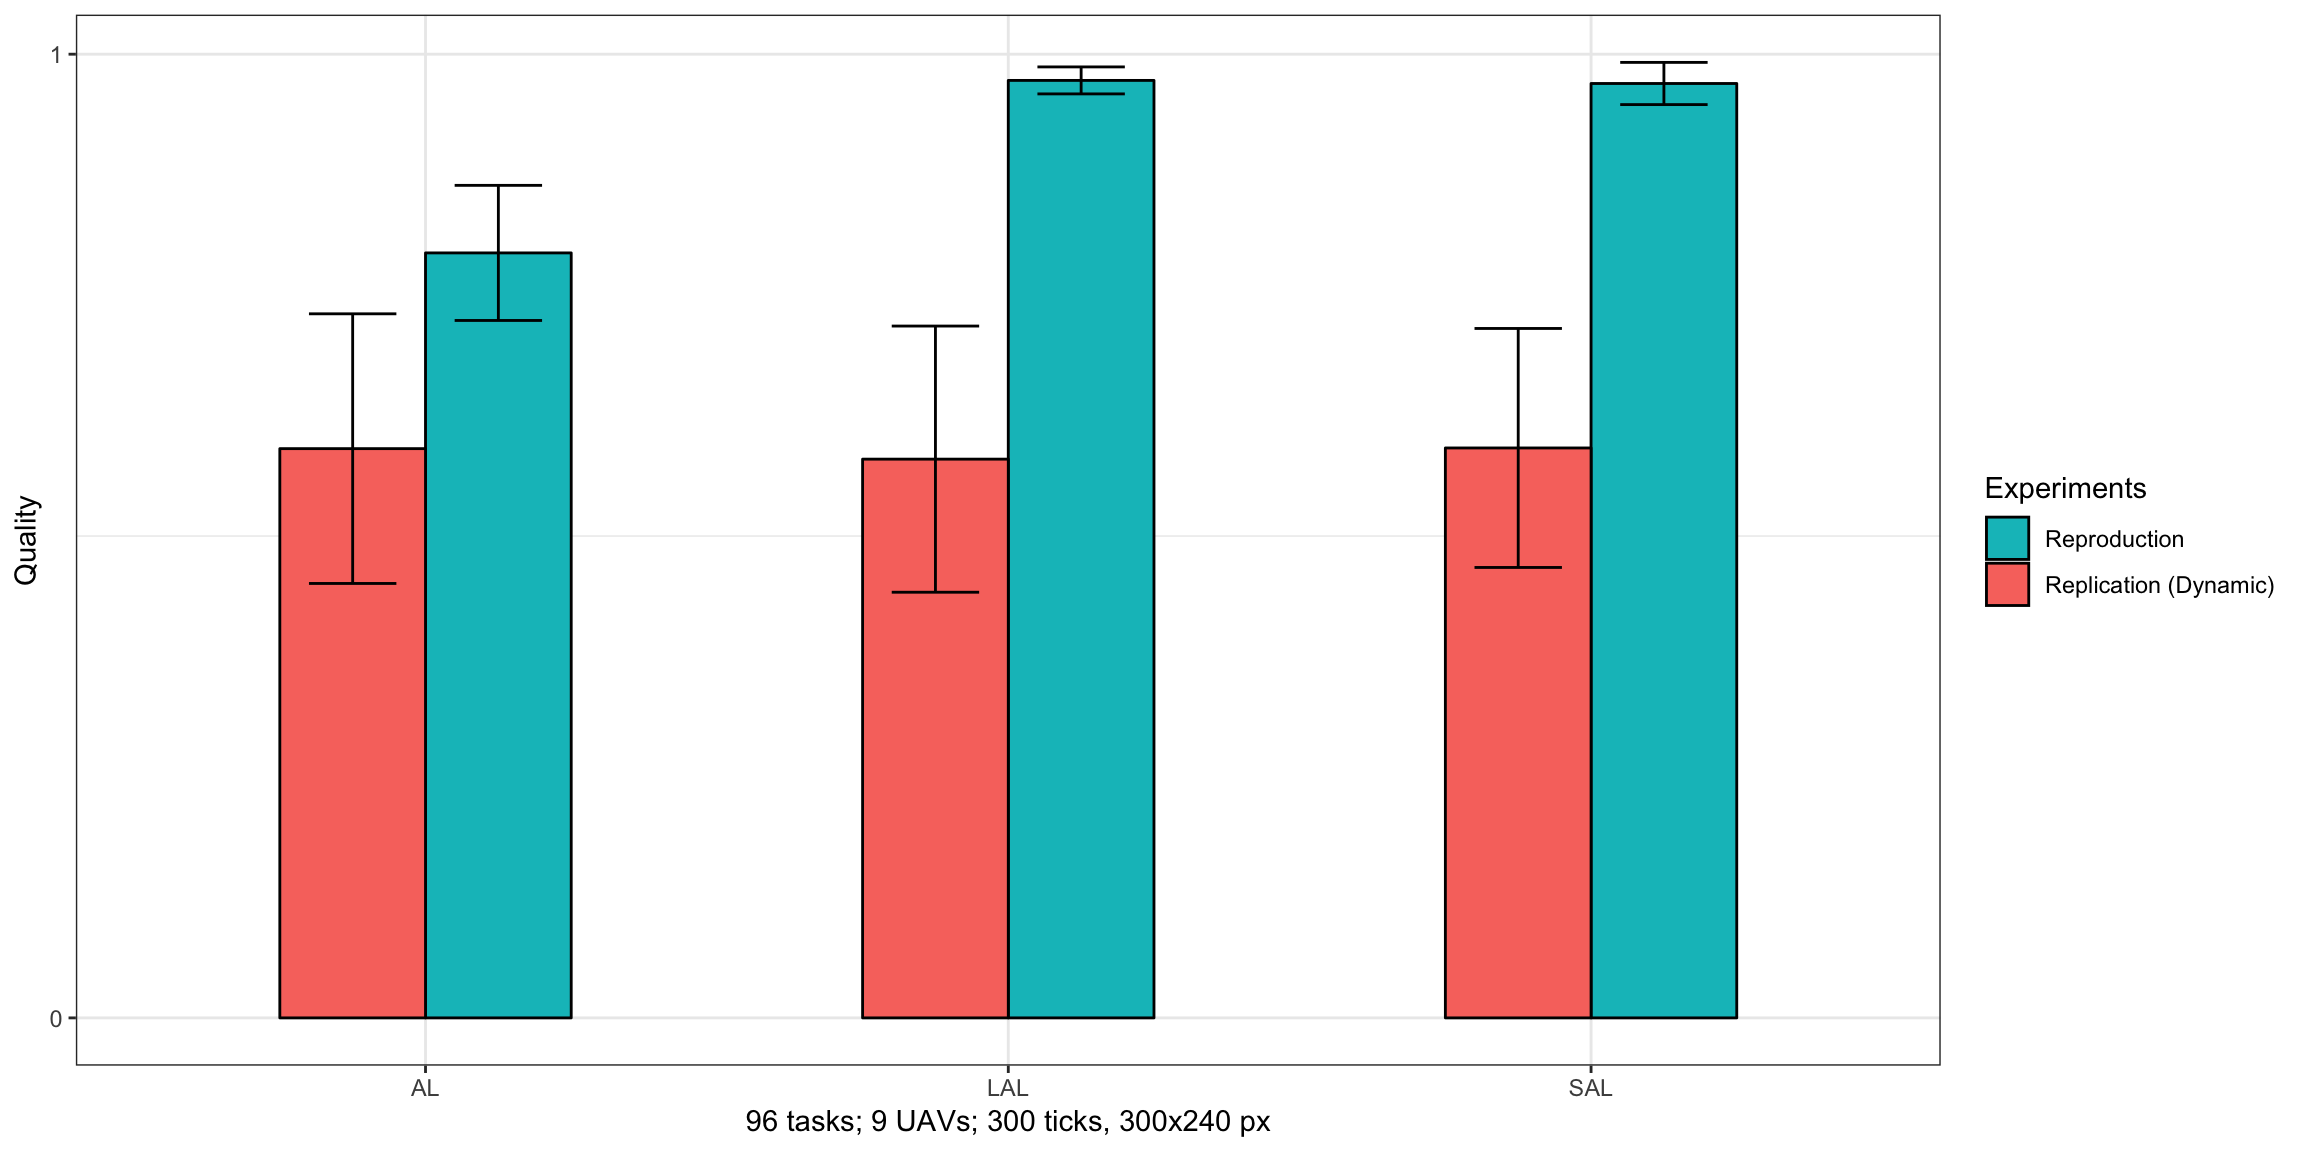
\includegraphics[scale=0.15]{fig/quality_orig.png}
		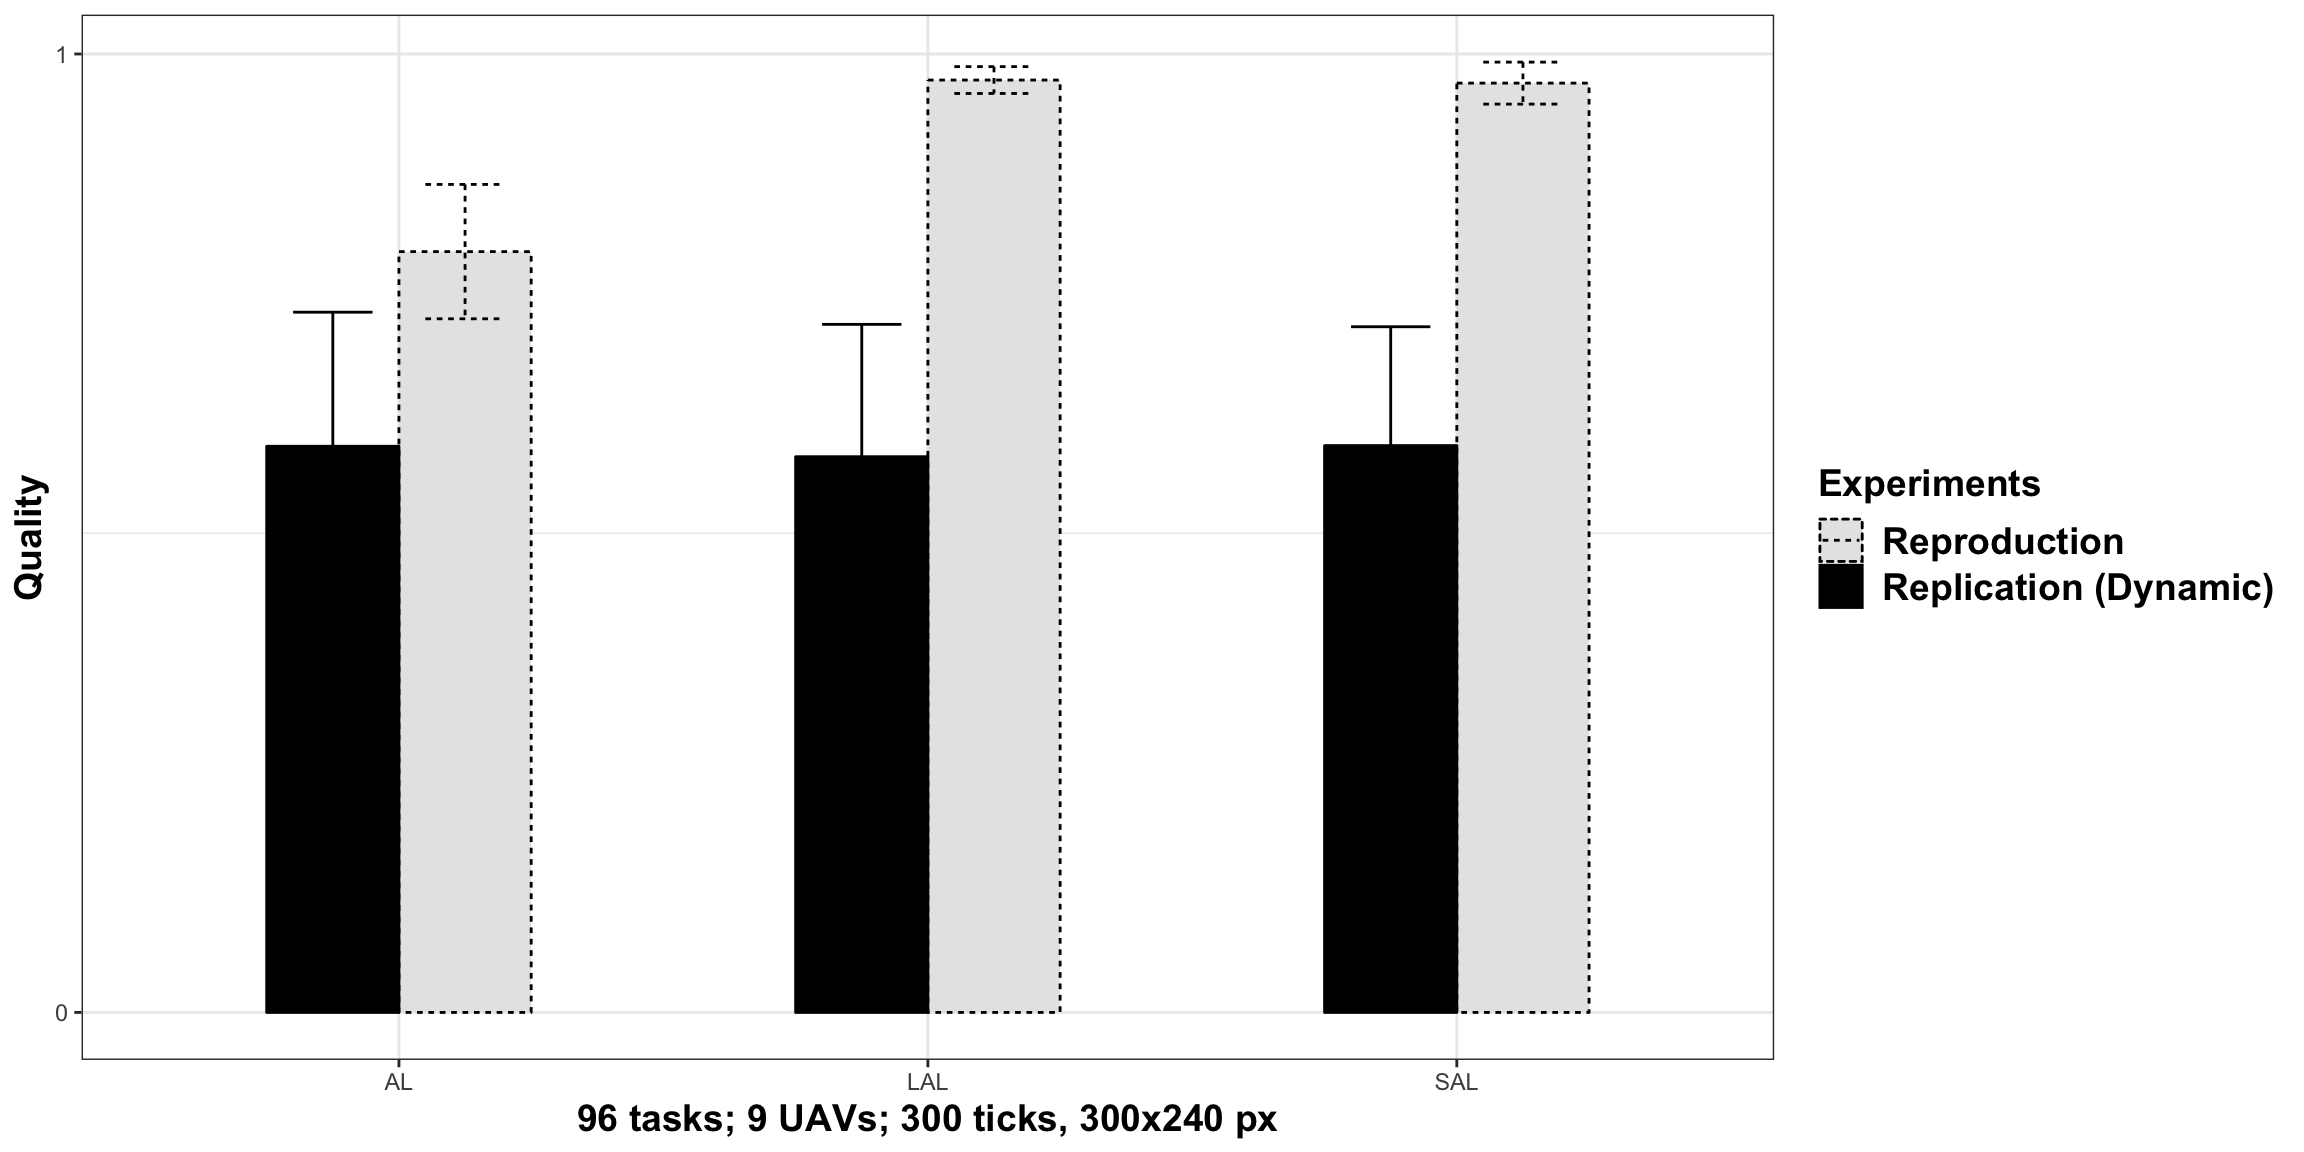
\includegraphics[scale=0.15]{fig/GRAPH02.png}
		\caption{Quality (96 tasks; 9 UAVs; 300 x 240; 300 ticks)}
		\label{fig:fig03}
	\end{center}
\end{figure}

On another hand, other metrics presented very similar results to the original experiment, as the number of messages exchanged, and the total reward and execution time.

The ring network relies on passing a token to each element. Even reducing the number of elements, the number of messages did not decrease because the token runs while it has tasks available or there is a UAV not visited by the token.

As the total reward is the sum of the UAV capability $k_{ij}$ related to the finished tasks, and the capability, defined in \citep{MAS07}, is a function of distance to the task and sensor quality, the reduction of quality causes a proportional decrease in the capability, as confirmed by Figure \ref{fig:fig02}.

\begin{figure}[h!]
	\begin{center}
		%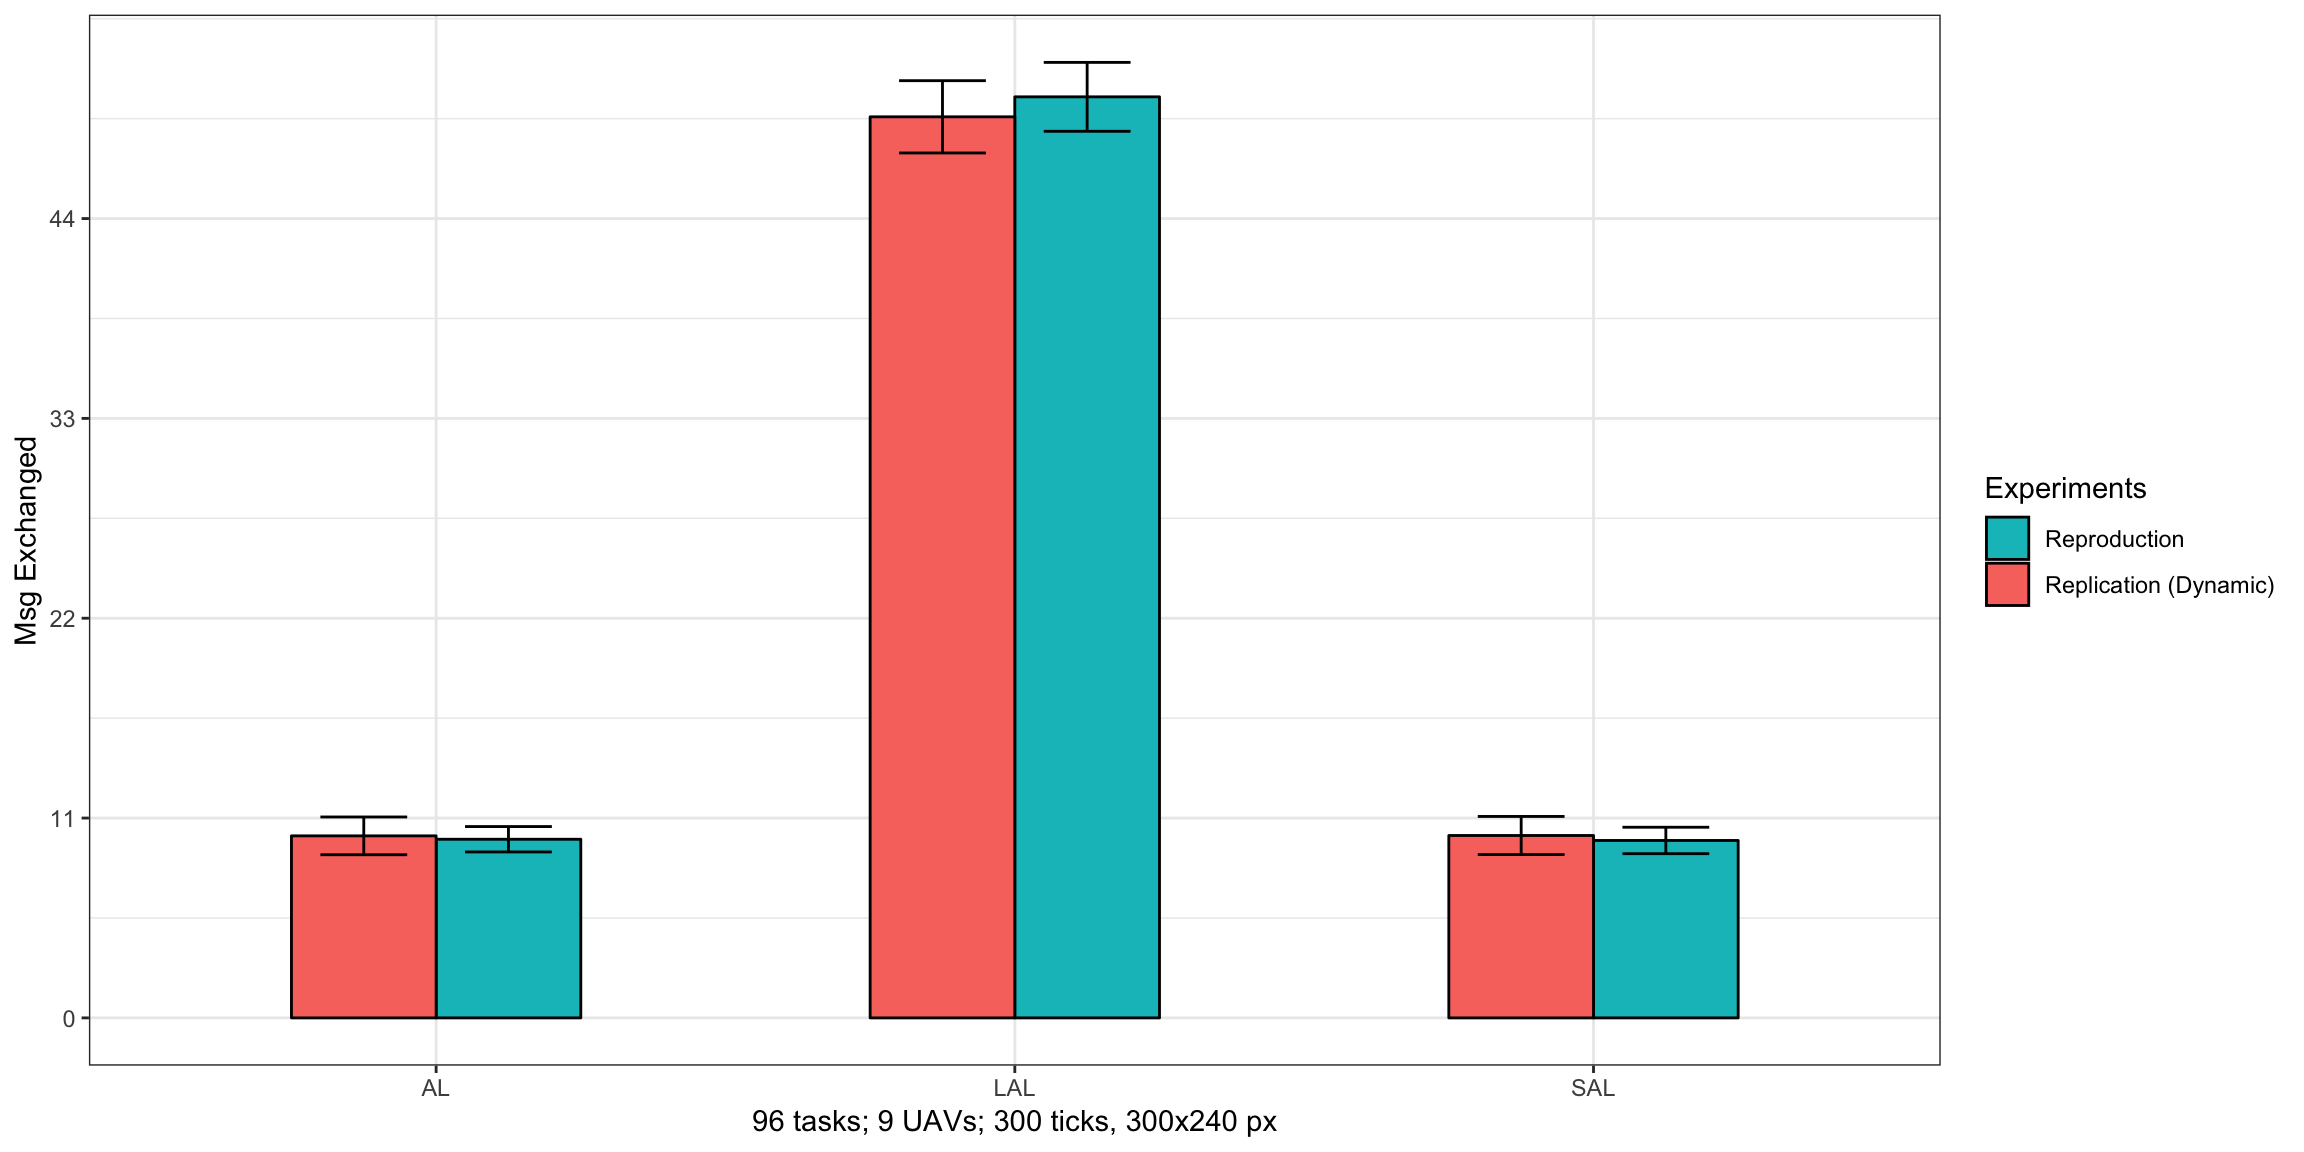
\includegraphics[scale=0.15]{fig/msg_orig.png}
		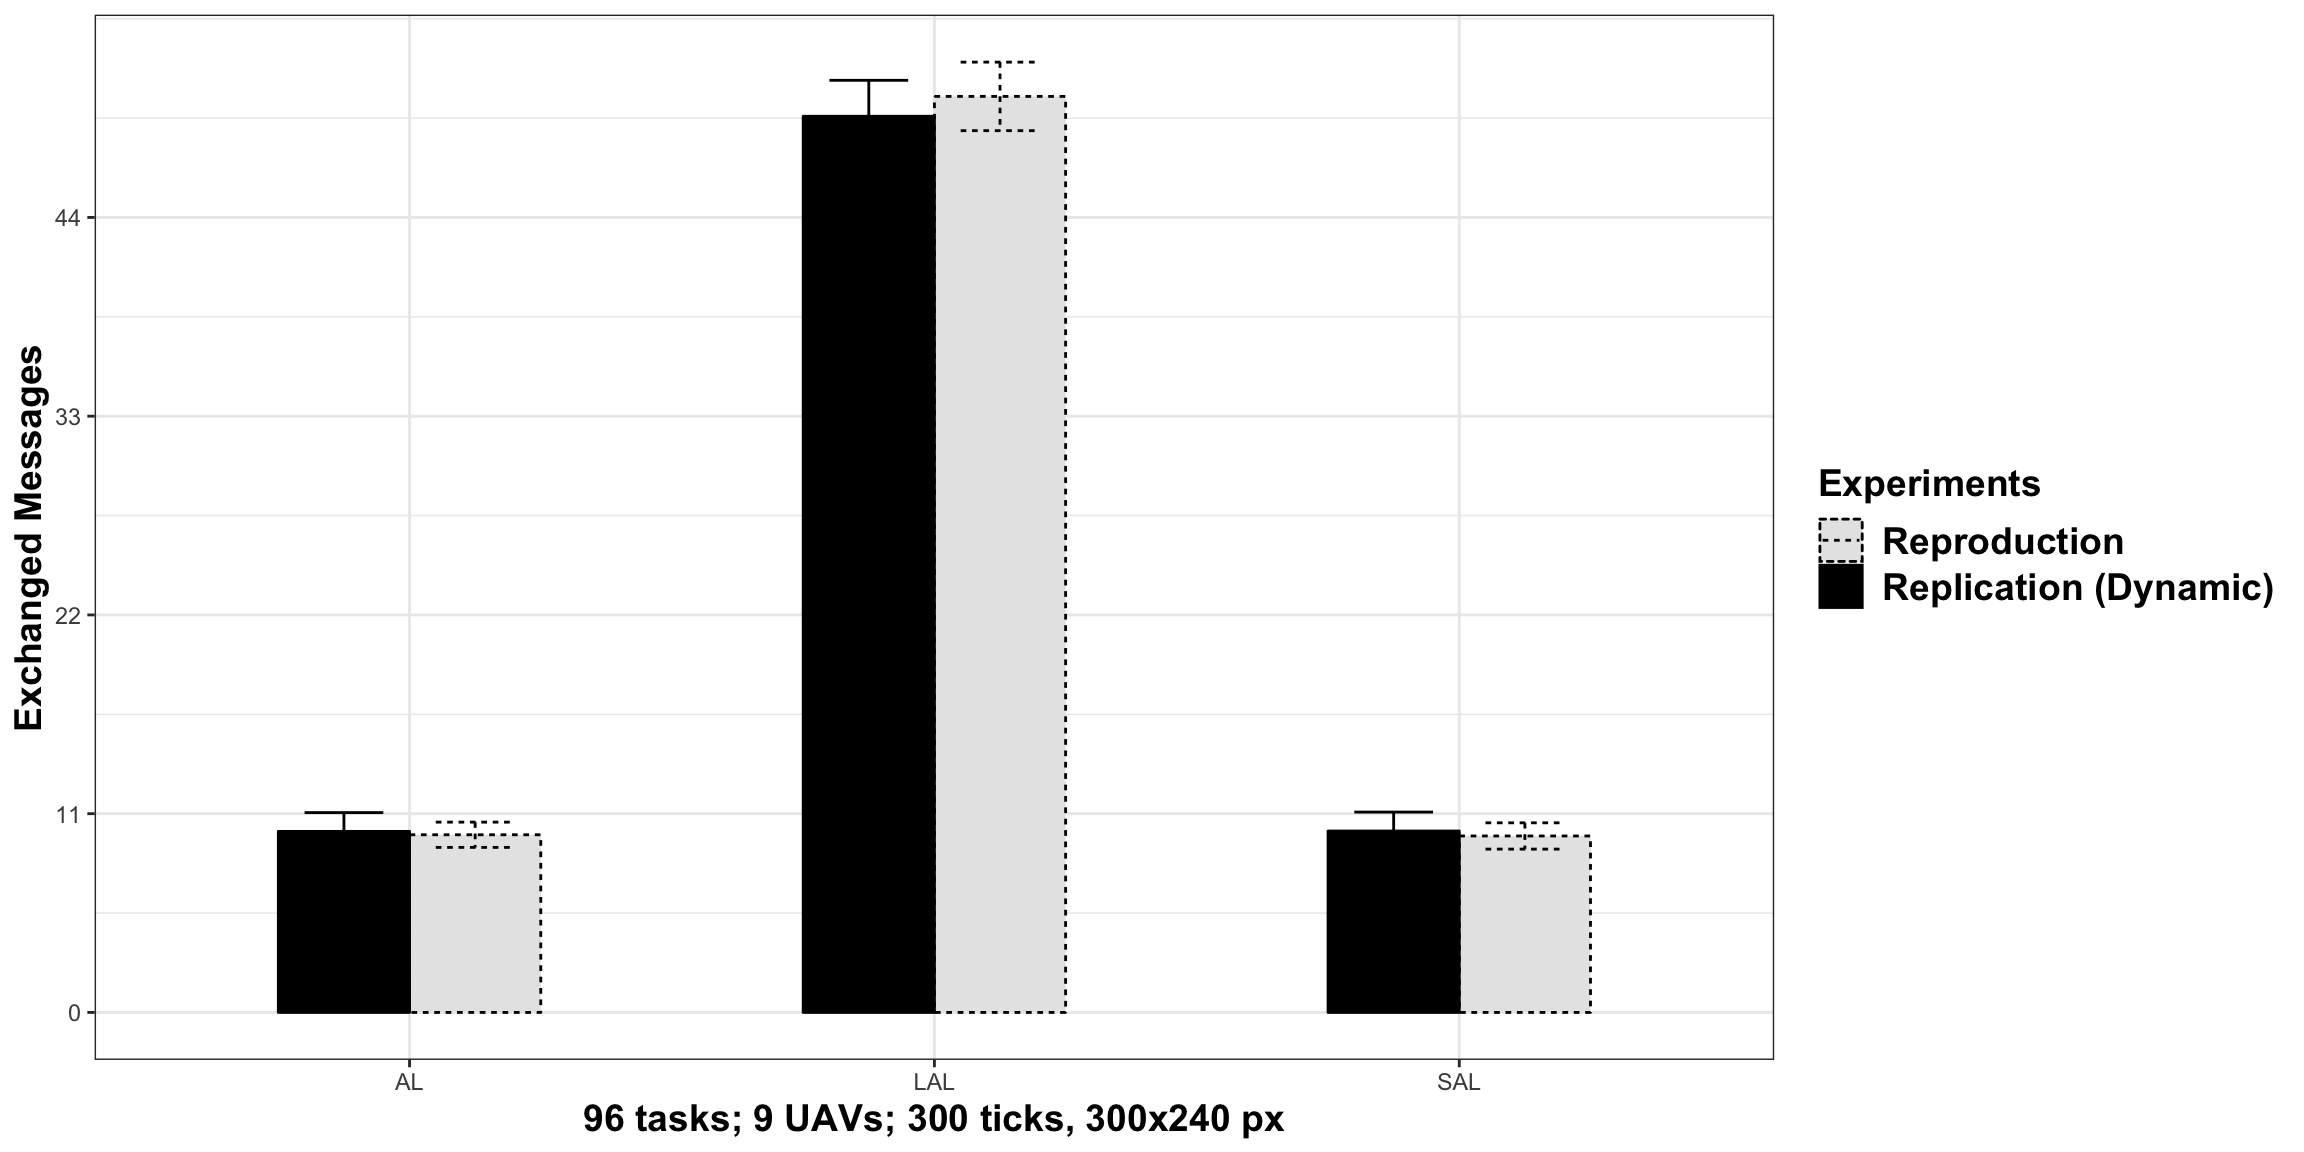
\includegraphics[scale=0.15]{fig/GRAPH03.png}
		\caption{Exchanged Messages  (96 tasks; 9 UAVs; 300 x 240; 300 ticks)}
		\label{fig:fig01}
	\end{center}
\end{figure}

\begin{figure}[h!]
	\begin{center}
		%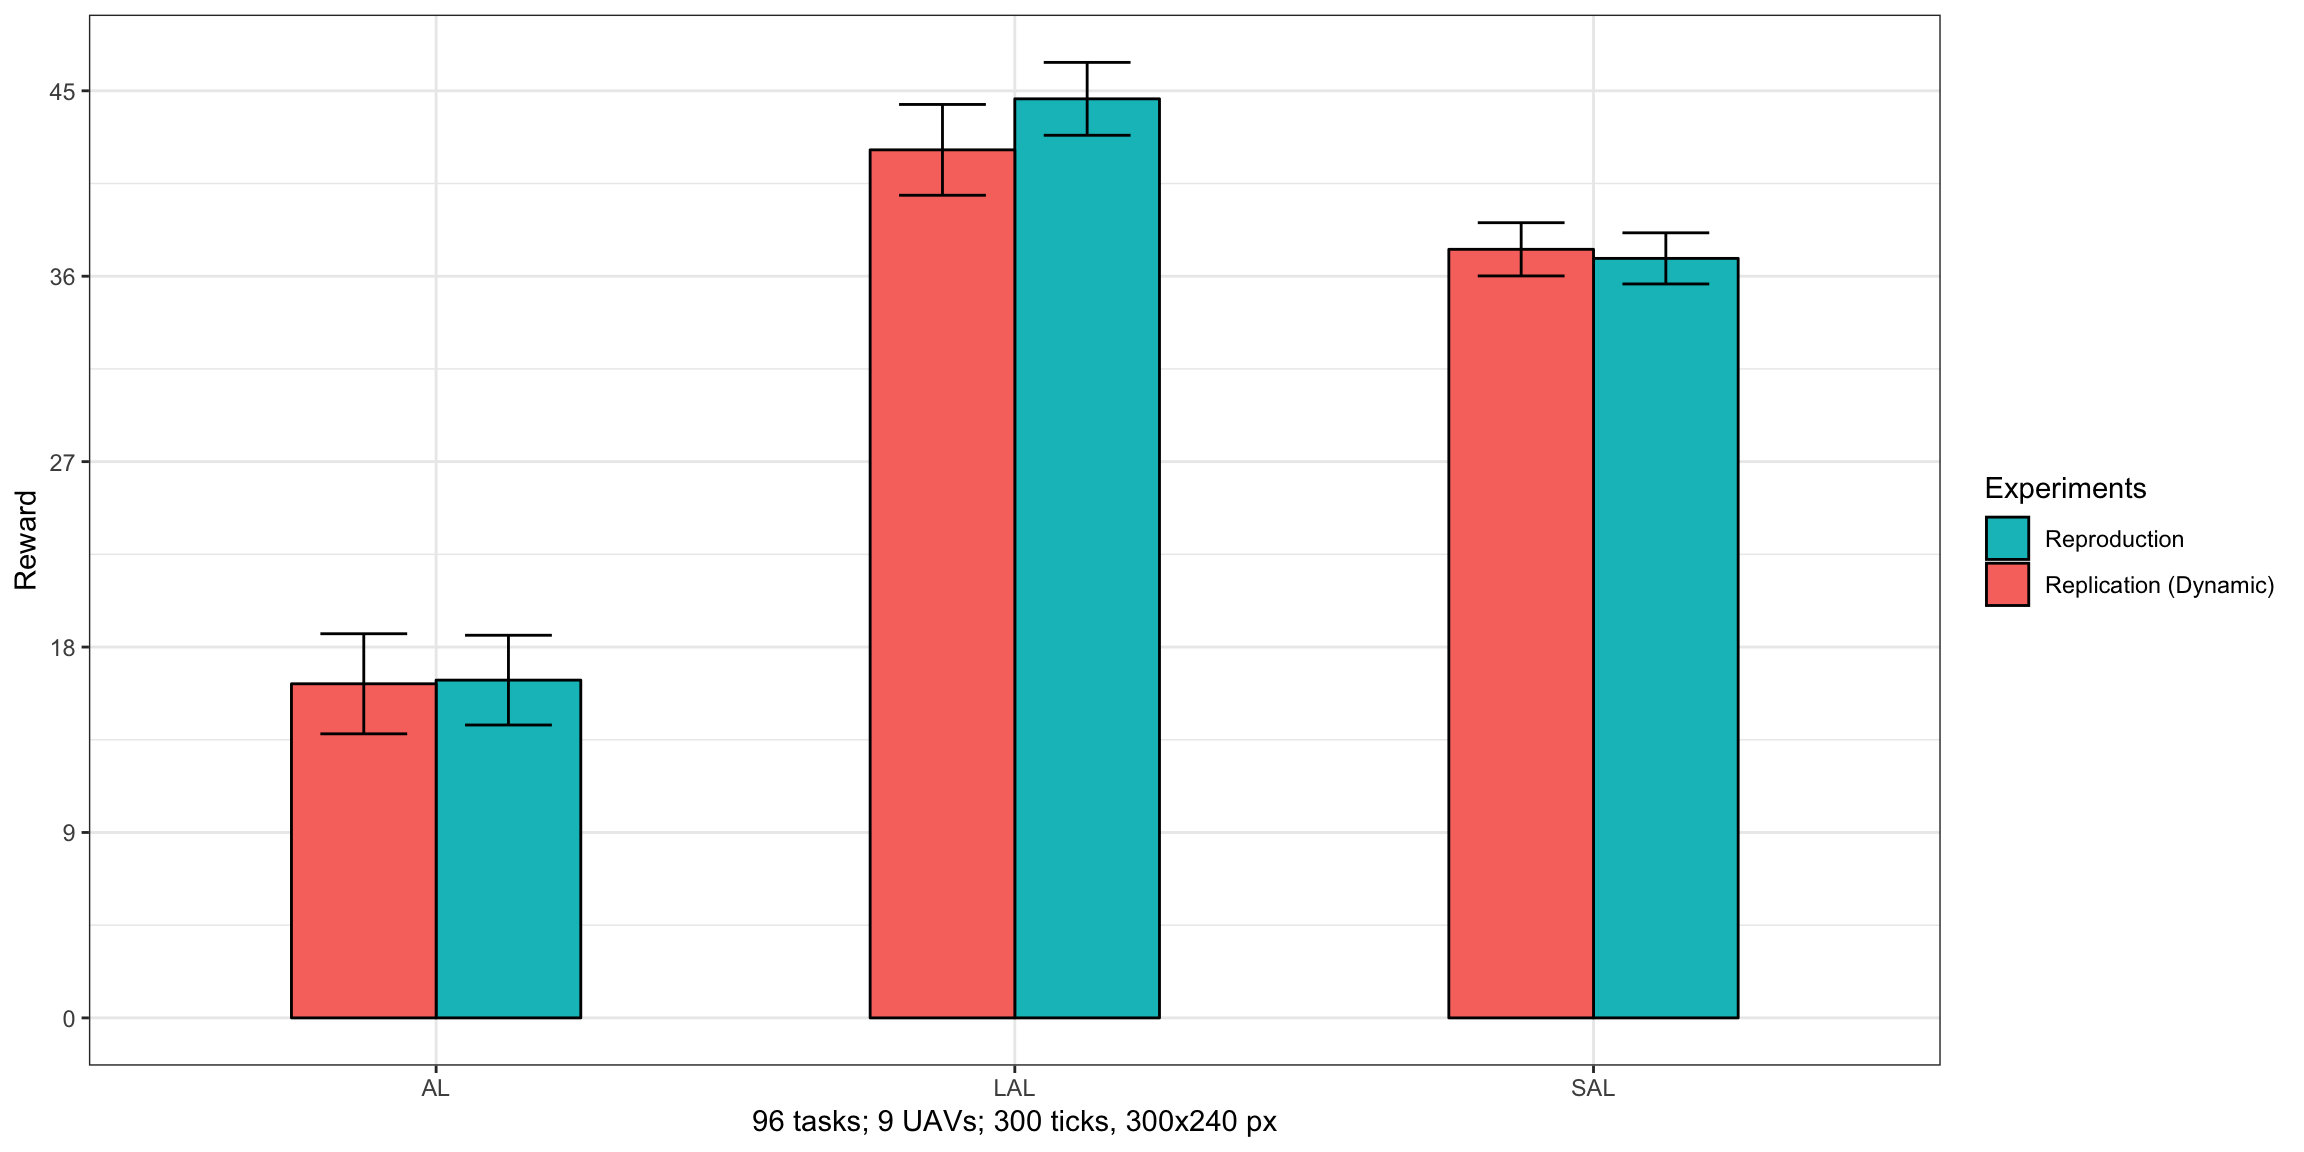
\includegraphics[scale=0.15]{fig/reward_orig.png}
		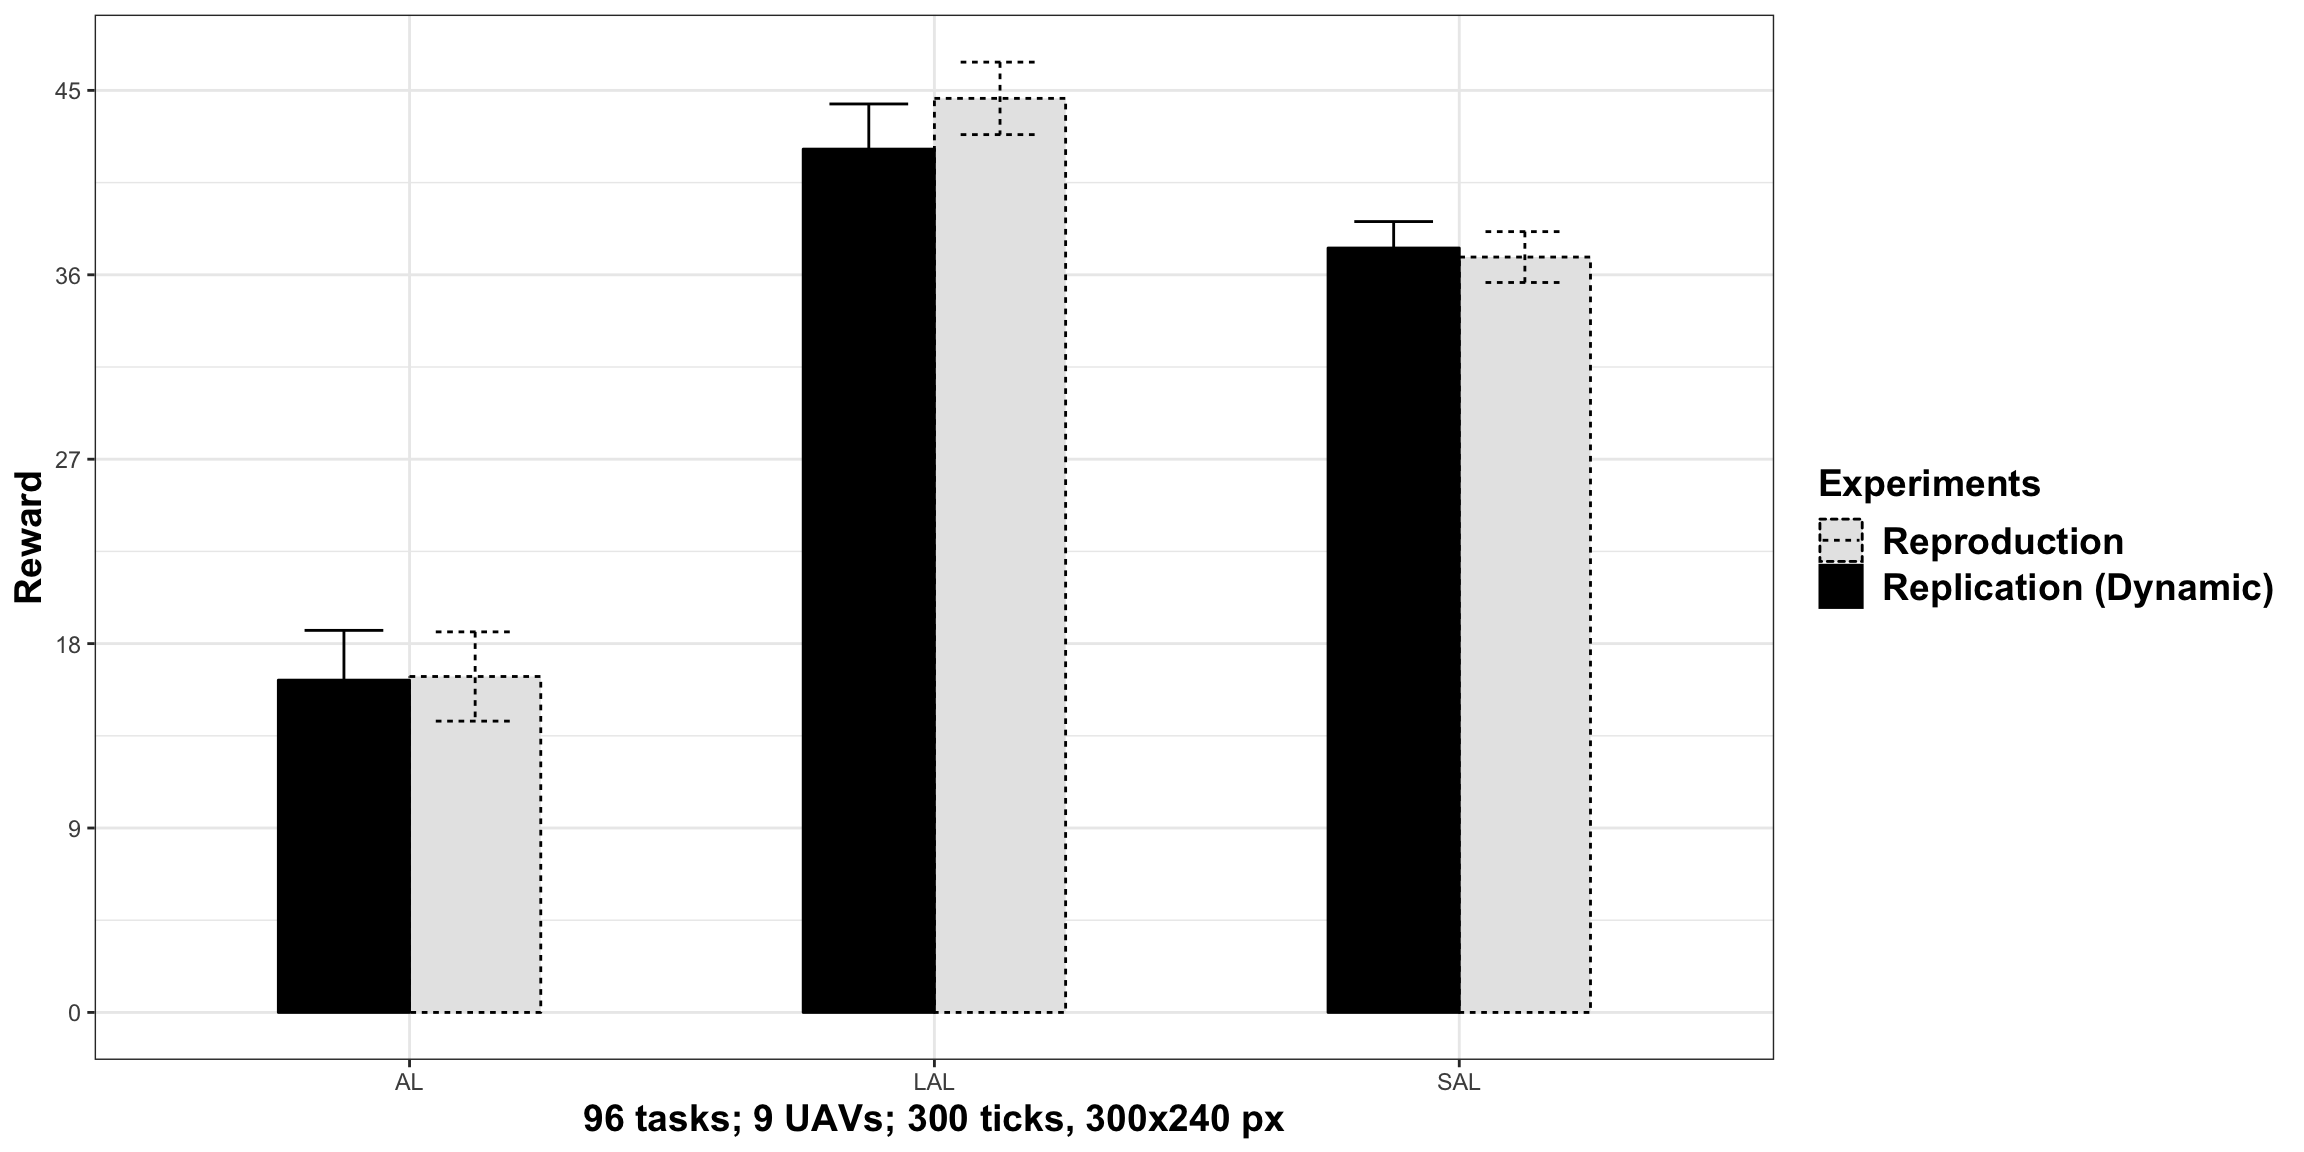
\includegraphics[scale=0.15]{fig/GRAPH04.png}
		\caption{Total Reward (96 tasks; 9 UAVs; 300 x 240; 300 ticks)}
		\label{fig:fig02}
	\end{center}
\end{figure}

\begin{figure}[h!]
	\begin{center}
		%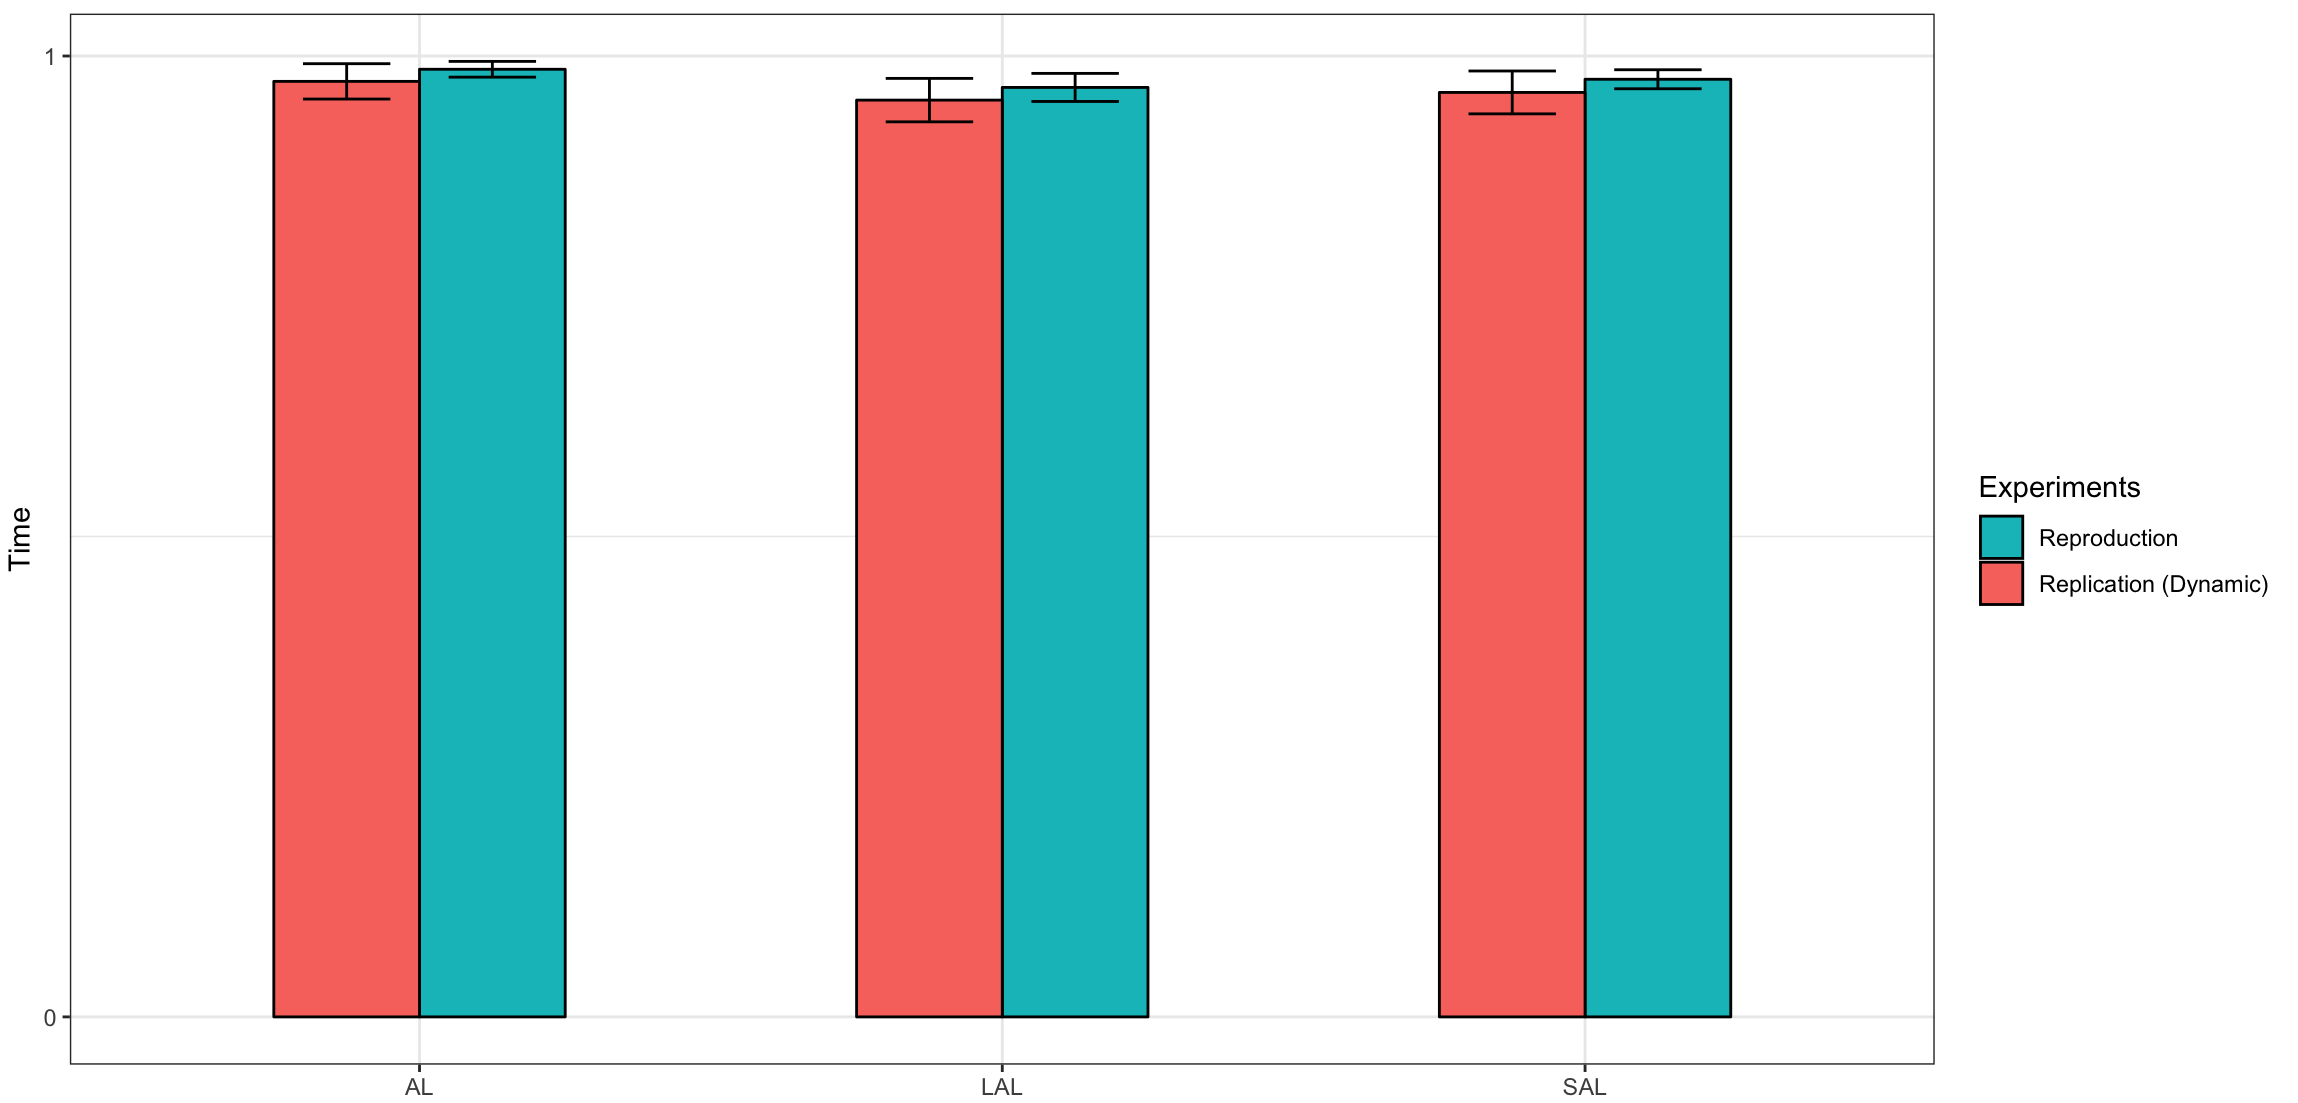
\includegraphics[scale=0.15]{fig/time_orig.png}
		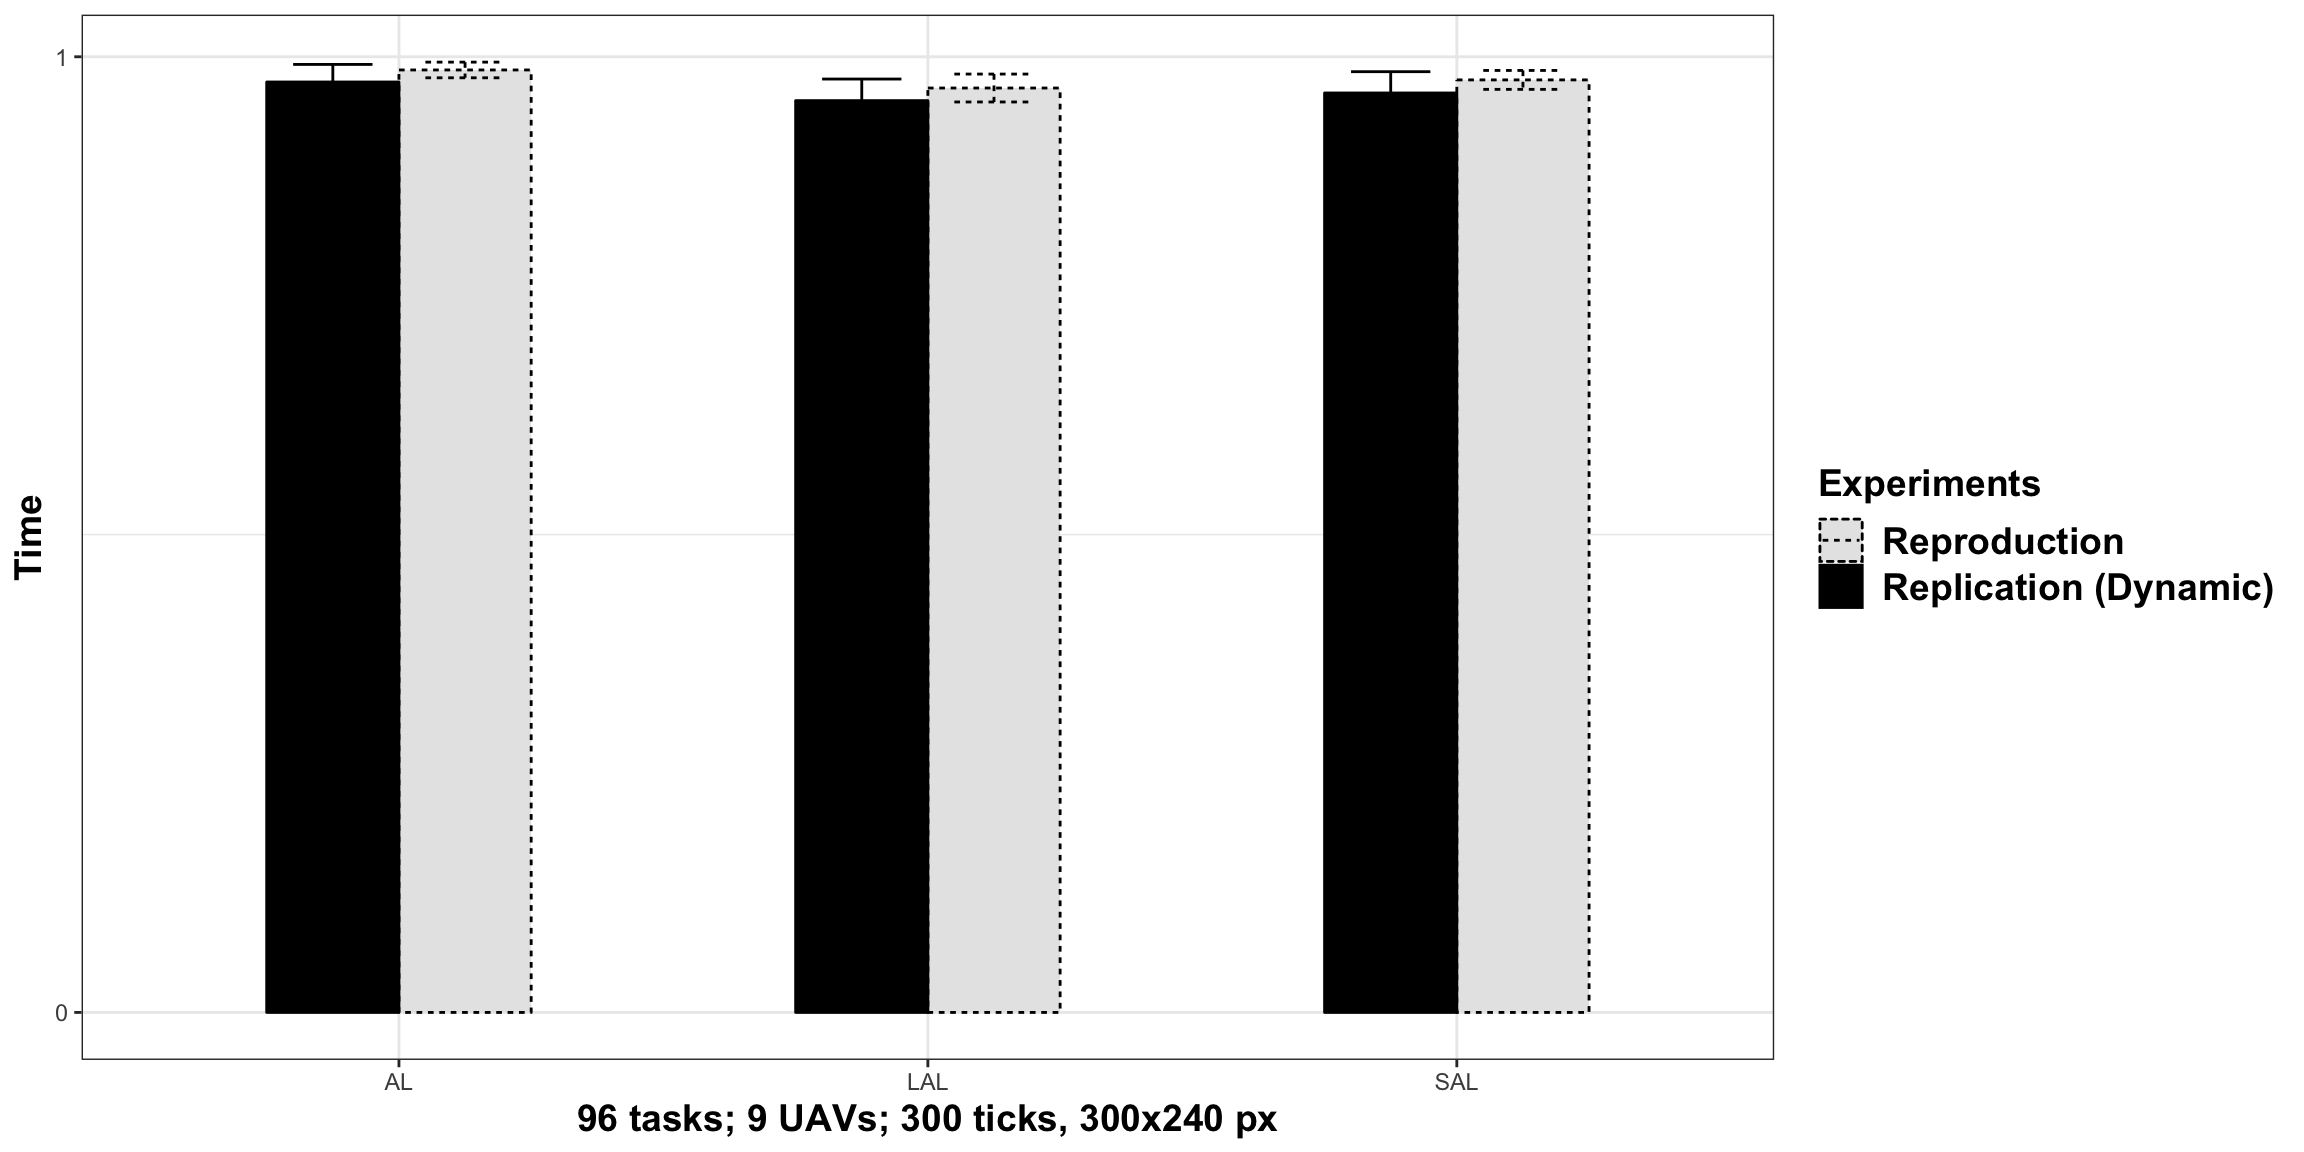
\includegraphics[scale=0.15]{fig/GRAPH05.png}
		\caption{Elapsed Time (96 tasks; 9 UAVs; 300 x 240; 300 ticks)}
		\label{fig:time}
	\end{center}
\end{figure}

The time measurement was done in percentage of total mission time (in ticks) utilization. The result obtained was equivalent to the original study experiments, considering the standard deviation (see Figure \ref{fig:time}). It is explained because the dynamic scenario ensures at least one UAV and this agent spends the most of the available time (in ticks) to execute the tasks allocated to it.

According to what was presented in~\citep{MAS07} and~\citep{ferreira2007swarm}, the more suitable value for $stimulus$ parameter is $0.6$. However, during the replications, different values were investigated. The resulting differences were not significant compared to those using the original $stimulus$ value in a static context reproduction. Therefore, all final results obtained in this section were based on the $stimulus = 0.6$